% Chapter 1

\chapter{Introduction} % Main chapter title

\label{Chapter1} % For referencing the chapter elsewhere, use \ref{Chapter1} 

%----------------------------------------------------------------------------------------
\section{Examples}

\lipsum[1-4]
\begin{shaded}
\noindent \textbf{Example:}
\lipsum[1]
\end{shaded}

\lipsum[5-6]

\section{Assumptions}
\begin{assumption} \label{ass:1}
	\lipsum[1]
\end{assumption}

\lipsum[1] 
\autoref{ass:1}

\section{Images}
\begin{figure}[h!]
	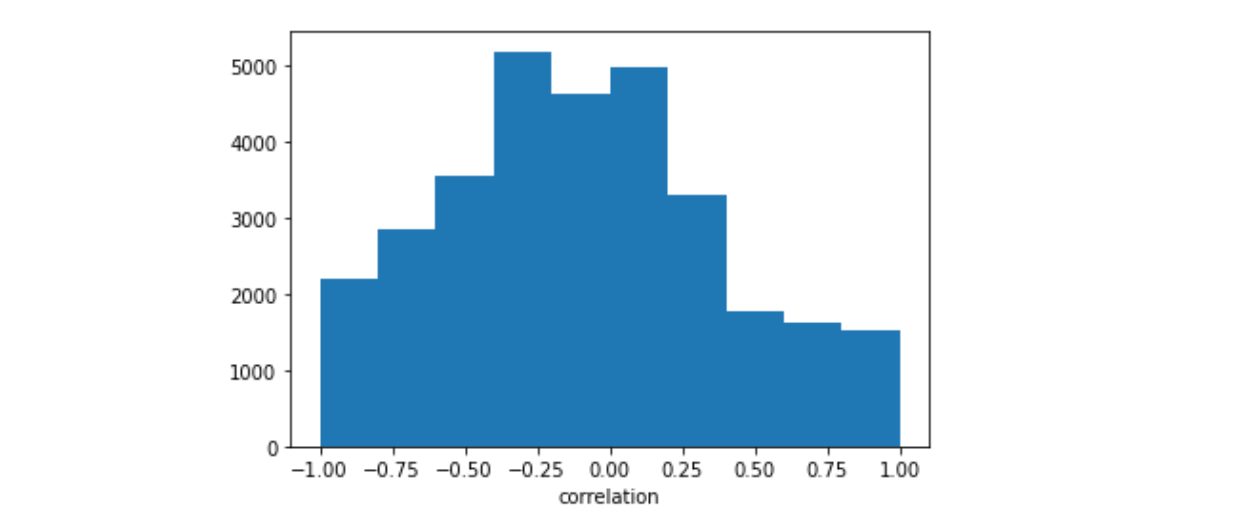
\includegraphics[width=\linewidth]{Figures/1.png}
	\caption{Histogram of item-wise correlations between stock and supply.}
	\label{fig:1}
\end{figure}
\lipsum[1] \autoref{fig:1}

\section{Equations}
\begin{equation} \label{eq:1}
	x=1
\end{equation}
\lipsum[1] \autoref{eq:1}

\section{Glossary Entries}
\lipsum[1]
\gls{glo1}

\section{Citation}
\lipsum[1]
\footcite{grimberg}


